\section{Application to color normalization}

Color normalization is the process of imposing the same color palette on a group of images. This color palette is always somehow related to the color palettes of the original images. For instance, if the goal is to cancel the illumination of a scene (avoid color cast), then the imposed histogram should be the histogram of the same scene illuminated with white light. Of course, in many occasions this information is not available. Following Papadakis et al.~\cite{Papadakis_ip11}, we define an in-between histogram, which is chosen here as the regularized OT barycenter. 

%The advantage with respect to Papadakis et al.'s method is that the influence of the input histograms on the barycenter can be easily tuned by a change of parameters, in fact it has as a special case any of the original image histograms. 

%Some other examples for which color normalization is useful are the color balancing of videos,  or as a preprocessing to register/compare several images taken with different cameras (see \cite{Papadakis_ip11} for more examples). 

%%%%%%%%%%%%%%%%%%%%%%%%%%%%%%%%%%%%%%%%%%%%%%%%%%%%%%%%%%%%%%%%%%
\subsection{Algorithm}

Given a set of input images $(X^{0[r]})_{r \in R}$, the goal is to impose on all the images the same histogram $\mu_X$ associated to the barycenter $X$. As for the colorization problem tackled in Section~\ref{sec-appli-color}, the first step is to subsample the original cloud of points $X^{0[r]}$ to make the problem tractable. Thus, for every $X^{0[r]}$ we compute a smaller associated point set $X^{[r]}$ using K-means clustering. Then, we obtain the barycenter $X$ of all the point clouds $(X^{[r]})_{r \in R}$ with the algorithms presented in Section~\ref{algobar}. Figure~\ref{im:baryillu} first row, shows an example on two synthetic cloud of points, $X^{[1]}$ in blue and $X^{[2]}$ in red. The cloud of points in green corresponds to the barycenter $X$, which can change its position depending on the parameter $\rho=(\rho_1,\rho_2)$ in~\eqref{eqbar} from $X^{[1]}$ for $\rho=(1,0)$ to $X^{[2]}$ when $\rho=(0,1)$.  This data set $X$ represents the 3-D histogram we want to impose on all the input images. 

Once we have $X$, we compute the regularized and relaxed OT transport maps $T^{[r]}$ between each $X^{[r]}$ and the barycenter $X$, by solving~\eqref{eq-symm-reg-energy}. The line segments in Figure~\ref{im:baryillu} represent the transport between point clouds, i.e. if $\Sig^{[1]}_{i,j}>0$, $X^{[1]}_i$ is linked to $X_j$, and similarly for $\Sig^{[2]}$. 

We apply $T^{[r]}$ to $X^{[r]}$, obtaining  $\tilde X^{[r]}$, for all $r \in R$, that is to say, we obtain a set of point clouds $\tilde X^{[r]}$ with a color distribution close to $X$.  Finally, to recover a set of high resolution images, we compute each $\tilde X^{0[r]}$ from $X^{0[r]}$ by up-sampling. A detailed description of the method is given in Algorithm~\ref{alg-norm}. 

\begin{algorithm}[ht!]
\caption{Regularized OT Color Normalization}
\label{alg-norm}
% \begin{algorithmic}[1]
\Require Images $\left( X^{0[r]} \right)_{r \in R} \in \RR^{N_0 \times d}$, $\la \in \RR^+ $, $\rho \in [0,1]^{|R|}$ and $k \in \RR^+$.

\Ensure Images $\left( \tilde X^{0[r]} \right)_{r \in R} \in \RR^{N_0 \times d}$.
% \Statex
\begin{enumerate}
	\algostep{Histogram down-sample} Compute $X^{[r]}$ from $X^{0[r]}$ using K-means clustering.
	\algostep{Compute barycenter} Compute with either~\eqref{eq-bar-l2} or~\eqref{eq-bar-l1} a barycenter $\mu_X$ where $X$ is a local minimum of~\eqref{eqbar} using the block coordinate descent described in Section~\ref{algobar}, see Algorithm~\ref{algo-block-barycenters}. 
	\algostep{Compute transport mappings} For all $r \in R$ compute $T^{[r]}$ between \\ 
		$X$ and $X^{[r]}$ by solving~\eqref{eq-symm-reg-energy}, such that $T^{[r]}(X^{[r]}_i) = Z^{[r]}_i$, where $Z^{[r]}= \diag(\Sig^{[r]} \U)^{-1} \Sig^{[r]} X$.
	\algostep{Transport up-sample} For every $T^{[r]}$ compute $\tilde T^{0[r]}$ following~\eqref{eq-upsample}.
	\algostep{Obtain high resolution results} Compute $\foralls r, \tilde X^{0[r]} = \tilde T^{0[r]}(X^{0[r]})$.
\end{enumerate}
% \end{algorithmic}
\end{algorithm}


%%%%%%%%%%%%%%%%%%%%%%%%%%%%%%%%%%%%%%%%%%%%%%%%%%%%%%%%%%%%%%%%%%
\subsection{Results}

We now show some example of color normalization using Algorithm~\ref{alg-norm}.

\begin{figure*}[!h]
\centering
\setlength{\arrayrulewidth}{2pt}
%%% OT %%%%
\begin{tabular}{@{}c@{\hspace{1mm}}c@{\hspace{1mm}}c@{\hspace{1mm}}c@{}}
	$\rho=(1,0)$ & $\rho=(0.7,0.3)$ & $\rho=(0.4,0.6)$ & $\rho=(0,1)$ \\
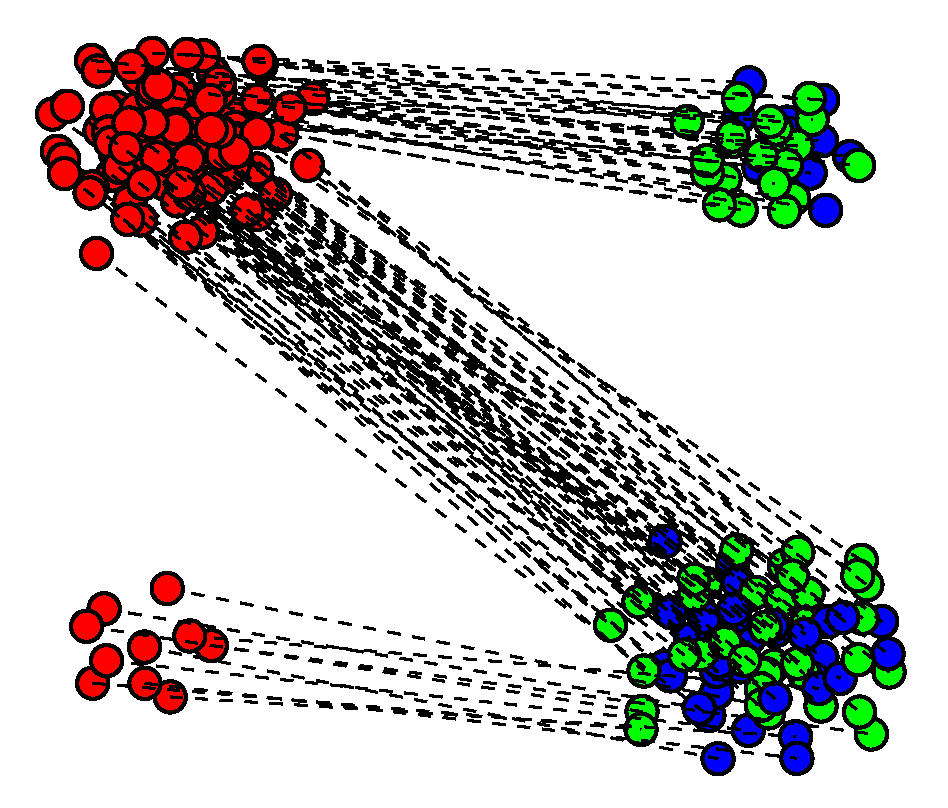
\includegraphics[width=.23\linewidth]{./syntheticbary/Barycenter_DiagsyntheticINVrho-0-ksum1lambda0nnx4QP1png} &  
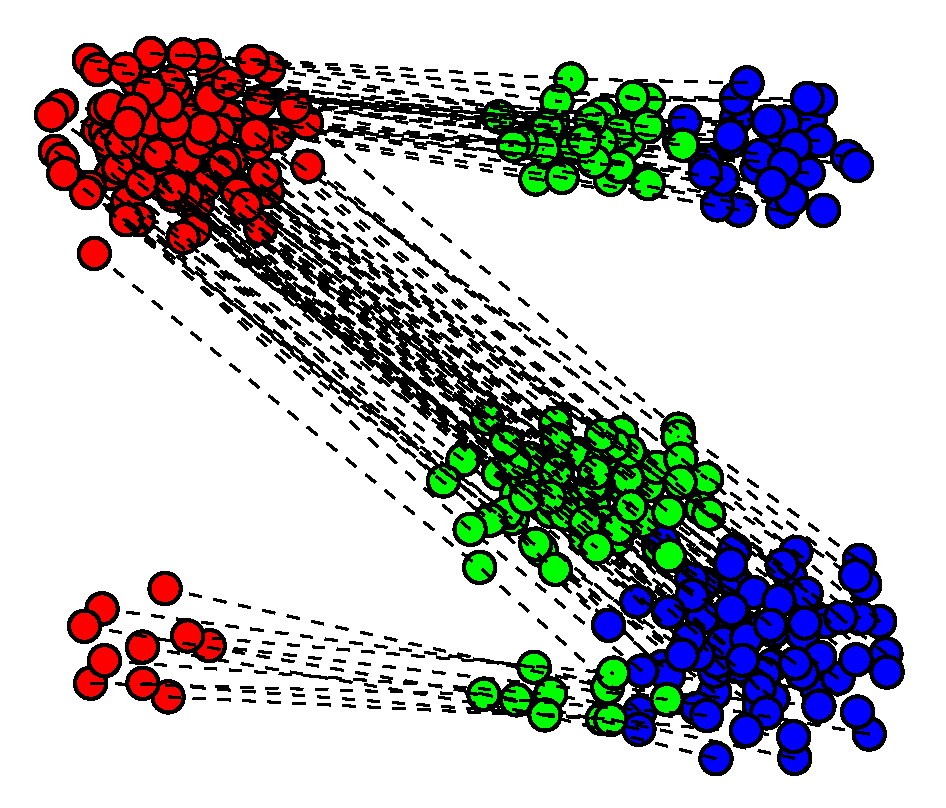
\includegraphics[width=.23\linewidth]{./syntheticbary/Barycenter_DiagsyntheticINVrho-03-ksum1lambda0nnx4QP1png} &
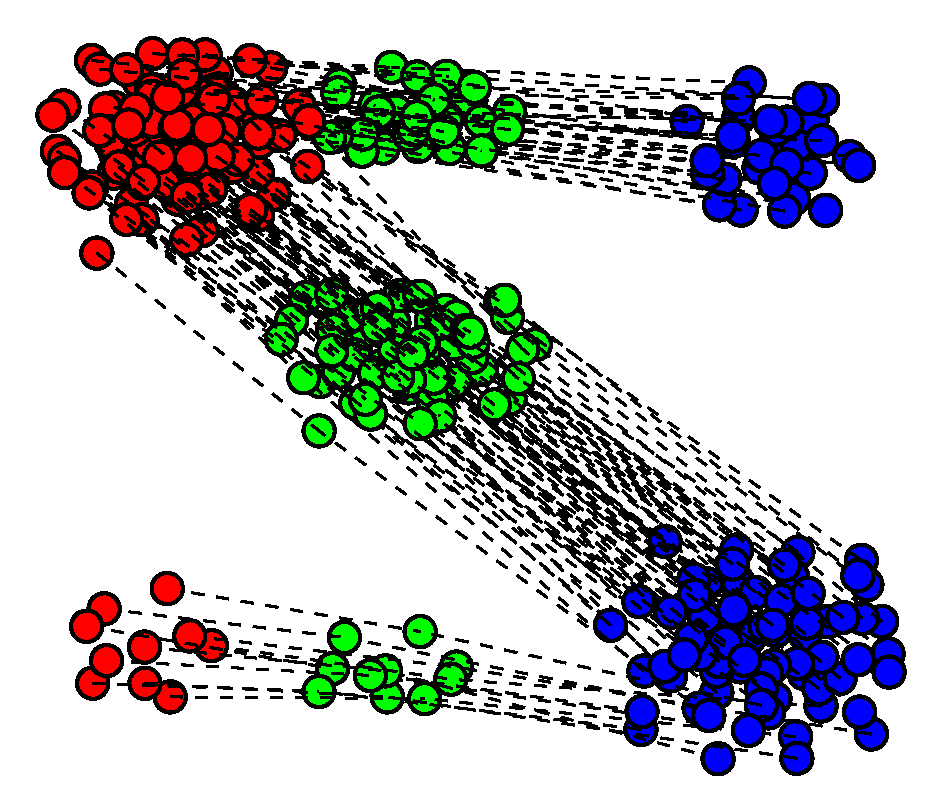
\includegraphics[width=.23\linewidth]{./syntheticbary/Barycenter_DiagsyntheticINVrho-06-ksum1lambda0nnx4QP1png} &
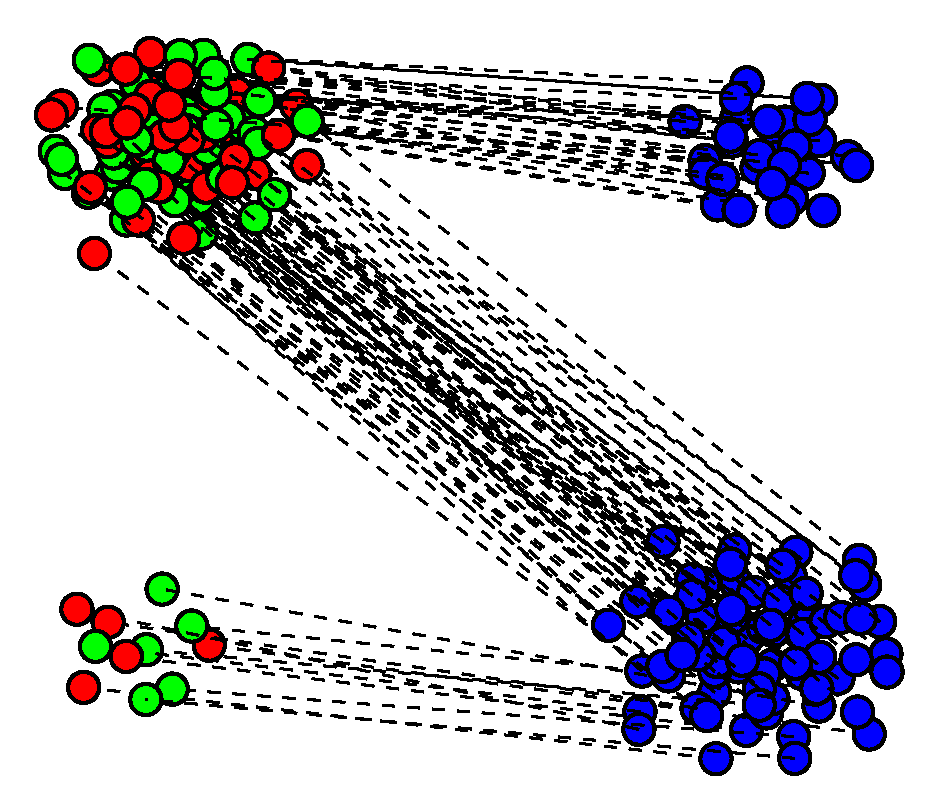
\includegraphics[width=.23\linewidth]{./syntheticbary/Barycenter_DiagsyntheticINVrho-1-ksum1lambda0nnx4QP1png} \\
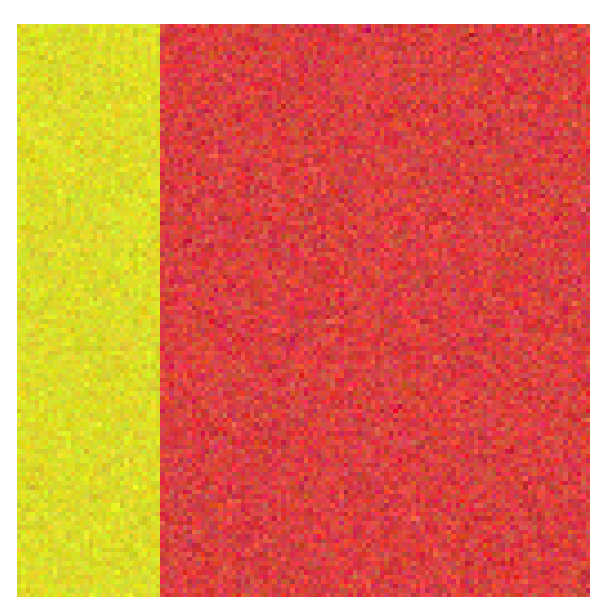
\includegraphics[width=.23\linewidth,height=.2\linewidth]{./syntheticbary/Diag2-syntheticrho-0-ksum1lambda0nnx4QP1} &
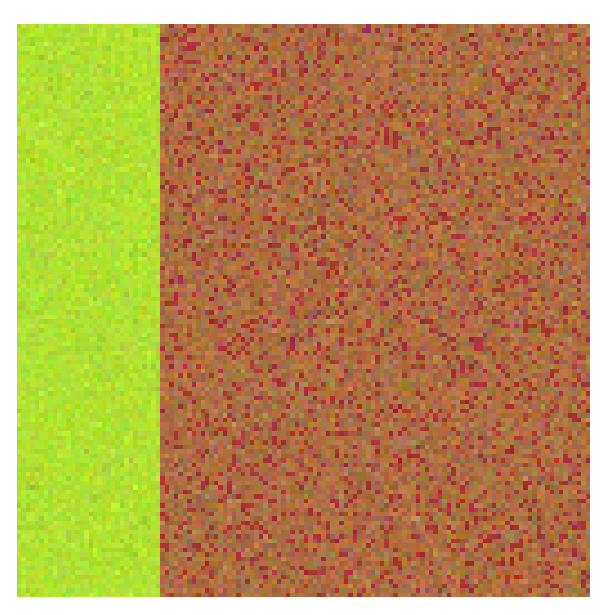
\includegraphics[width=.23\linewidth,height=.2\linewidth]{./syntheticbary/Diag2-syntheticrho-03-ksum1lambda0nnx4QP1} &
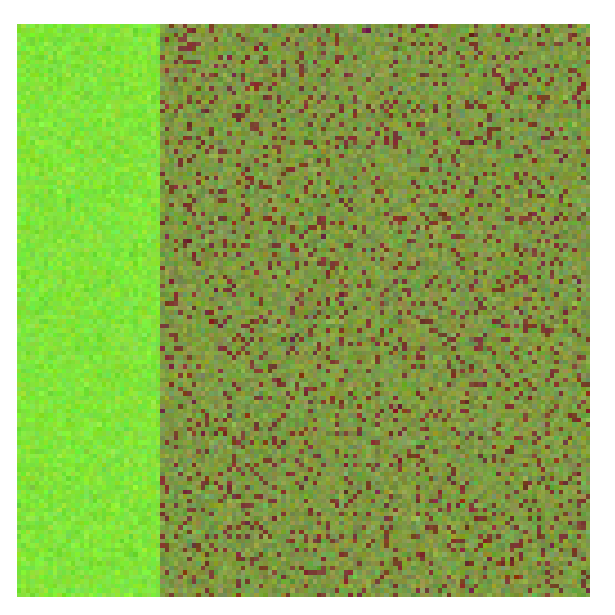
\includegraphics[width=.23\linewidth,height=.2\linewidth]{./syntheticbary/Diag2-syntheticrho-06-ksum1lambda0nnx4QP1} &
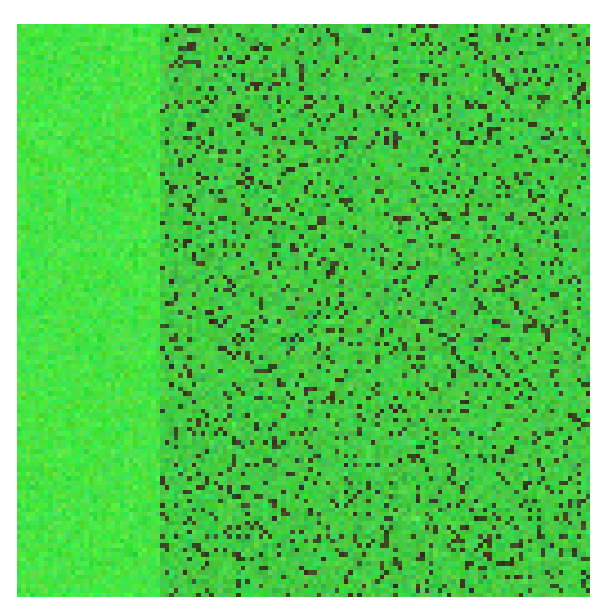
\includegraphics[width=.23\linewidth,height=.2\linewidth]{./syntheticbary/Diag2-syntheticrho-1-ksum1lambda0nnx4QP1}\\
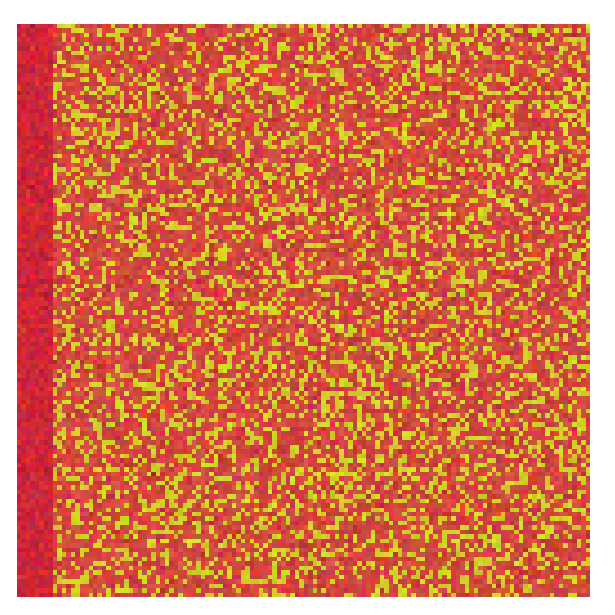
\includegraphics[width=.23\linewidth,height=.2\linewidth]{./syntheticbary/Diag1-syntheticrho-0-ksum1lambda0nnx4QP1} &
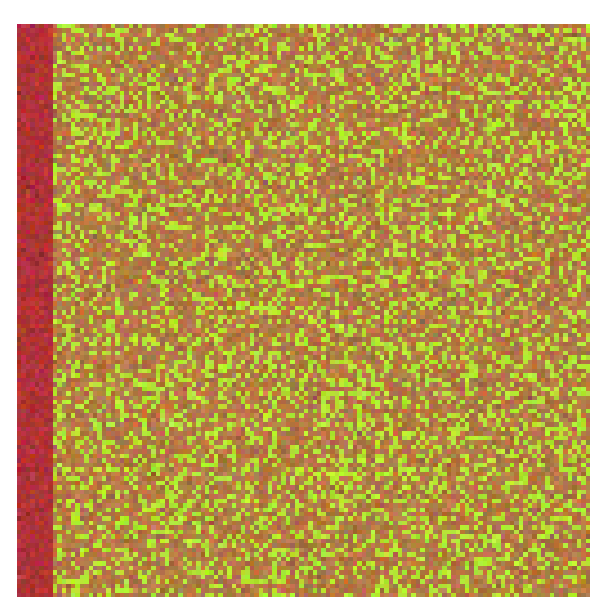
\includegraphics[width=.23\linewidth,height=.2\linewidth]{./syntheticbary/Diag1-syntheticrho-03-ksum1lambda0nnx4QP1} &
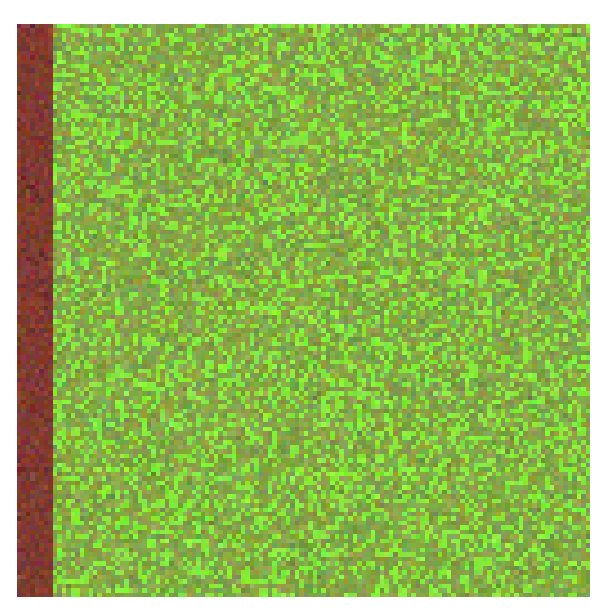
\includegraphics[width=.23\linewidth,height=.2\linewidth]{./syntheticbary/Diag1-syntheticrho-06-ksum1lambda0nnx4QP1} &
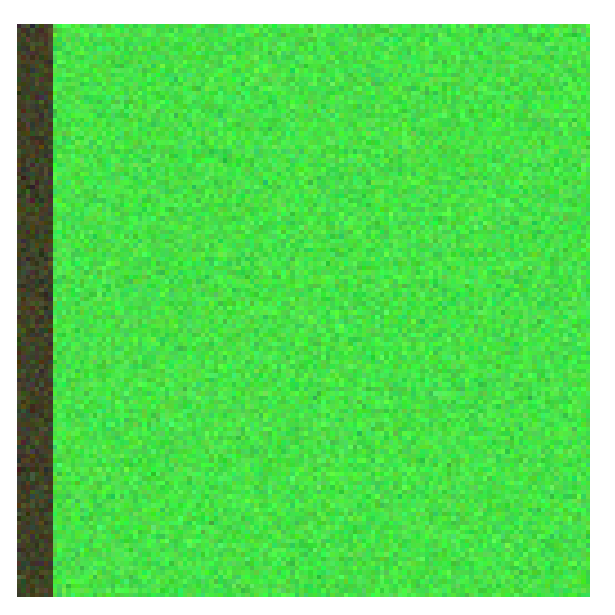
\includegraphics[width=.23\linewidth,height=.2\linewidth]{./syntheticbary/Diag1-syntheticrho-1-ksum1lambda0nnx4QP1} \\\hline
%%% Regularized
\includegraphics[width=.23\linewidth]{./syntheticbary/Barycenter_DiagsyntheticINVrho-0-ksum20lambda00005nnx4QP1} &
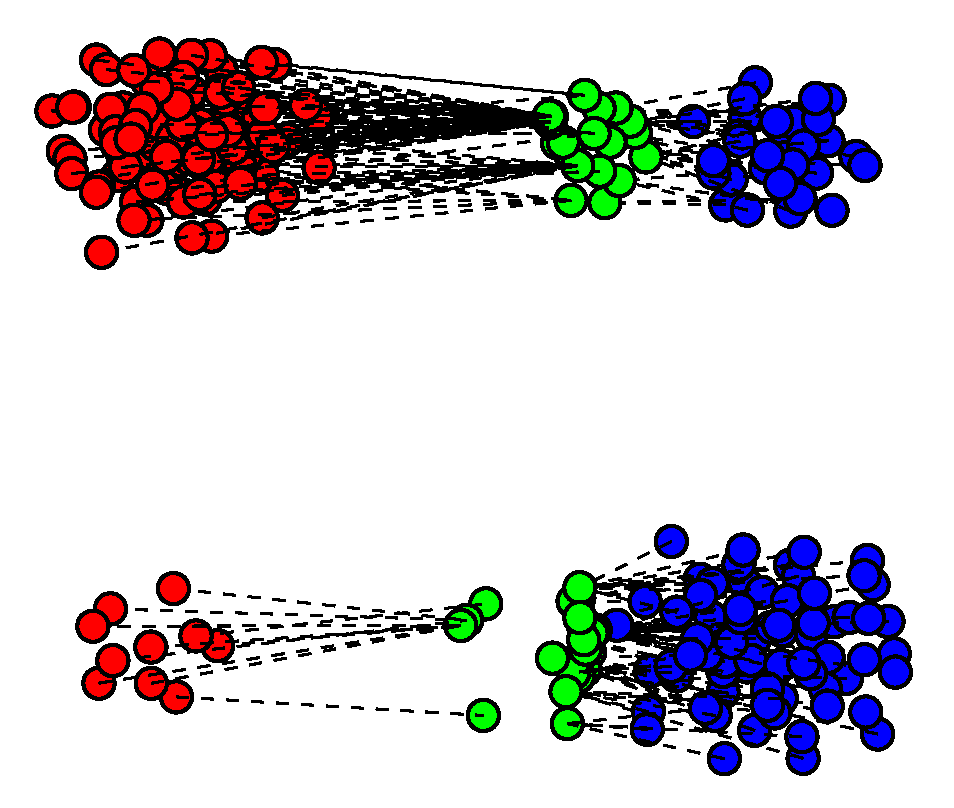
\includegraphics[width=.23\linewidth]{./syntheticbary/Barycenter_DiagsyntheticINVrho-03-ksum20lambda00005nnx4QP1} & 
\includegraphics[width=.23\linewidth]{./syntheticbary/Barycenter_DiagsyntheticINVrho-06-ksum20lambda00005nnx4QP1} &
\includegraphics[width=.23\linewidth]{./syntheticbary/Barycenter_DiagsyntheticINVrho-1-ksum20lambda00005nnx4QP1} \\
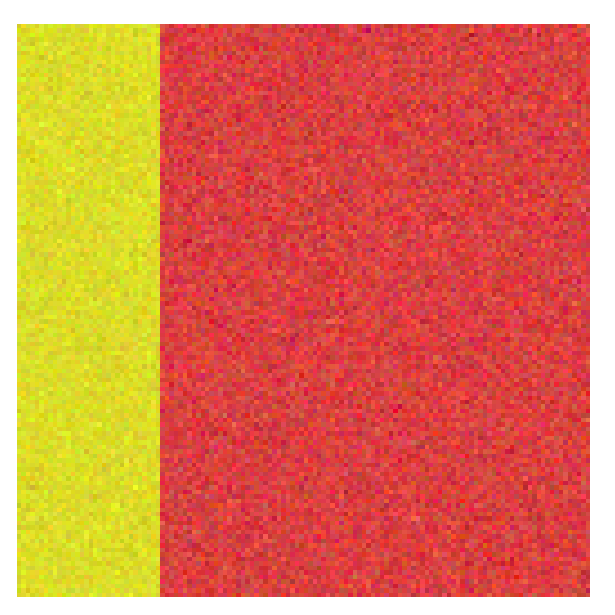
\includegraphics[width=.23\linewidth,height=.2\linewidth]{./syntheticbary/Diag2-syntheticrho-01-ksum20lambda00005nnx4QP1} &
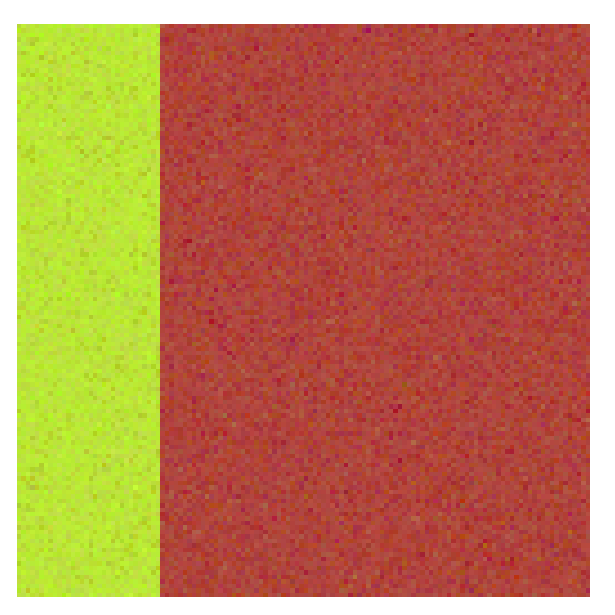
\includegraphics[width=.23\linewidth,height=.2\linewidth]{./syntheticbary/Diag2-syntheticrho-0307-ksum20lambda00005nnx4QP1}& 
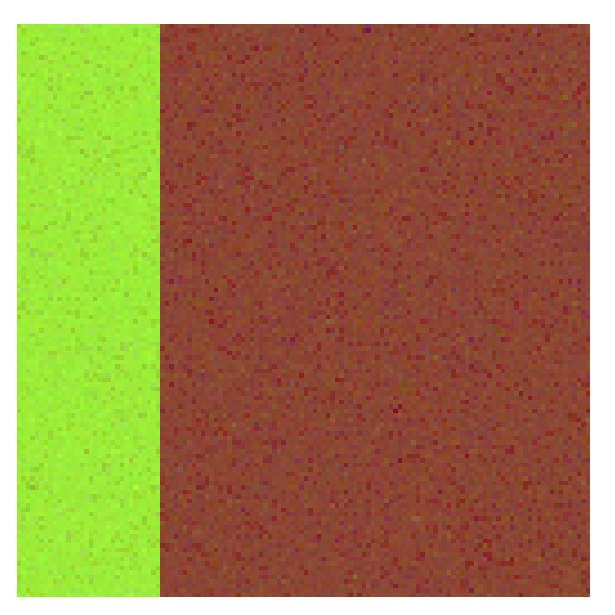
\includegraphics[width=.23\linewidth,height=.2\linewidth]{./syntheticbary/Diag2-syntheticrho-0604-ksum20lambda00005nnx4QP1} &
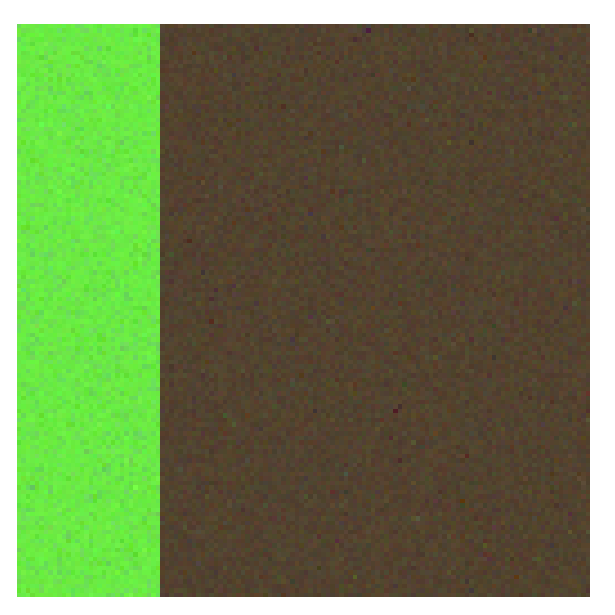
\includegraphics[width=.23\linewidth,height=.2\linewidth]{./syntheticbary/Diag2-syntheticrho-10-ksum20lambda00005nnx4QP1}\\
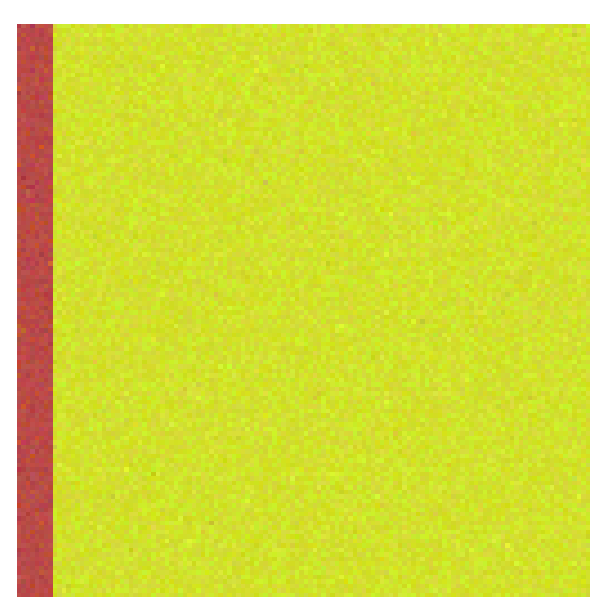
\includegraphics[width=.23\linewidth,height=.2\linewidth]{./syntheticbary/Diag1-syntheticrho-01-ksum20lambda00005nnx4QP1} &
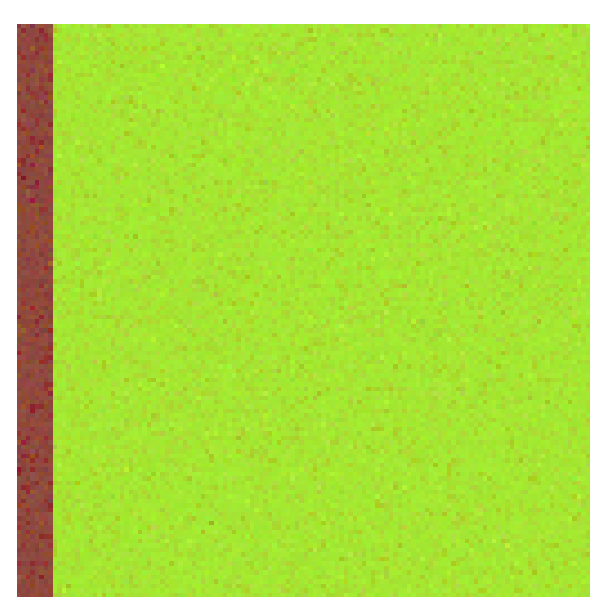
\includegraphics[width=.23\linewidth,height=.2\linewidth]{./syntheticbary/Diag1-syntheticrho-0307-ksum20lambda00005nnx4QP1} & 
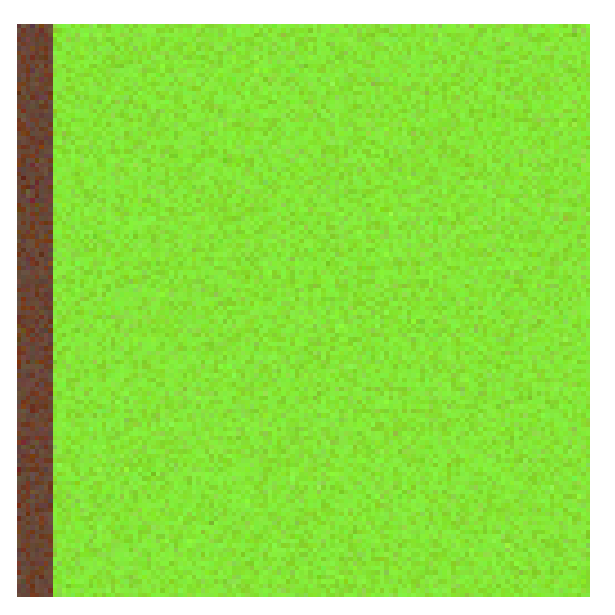
\includegraphics[width=.23\linewidth,height=.2\linewidth]{./syntheticbary/Diag1-syntheticrho-0604-ksum20lambda00005nnx4QP1} &
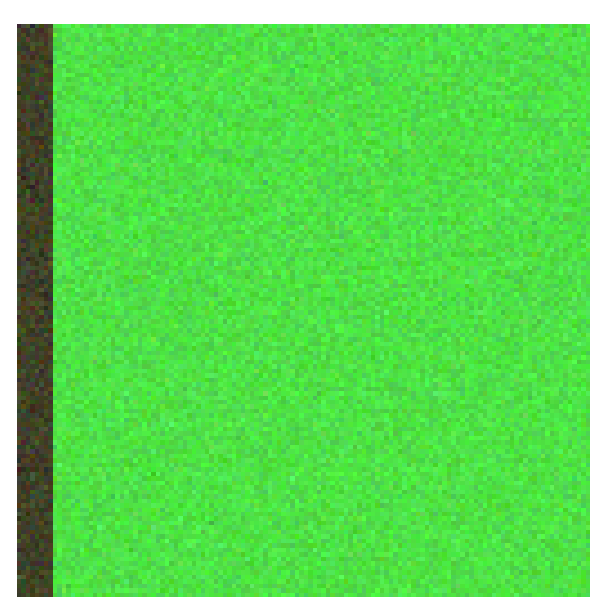
\includegraphics[width=.23\linewidth,height=.2\linewidth]{./syntheticbary/Diag1-syntheticrho-10-ksum20lambda00005nnx4QP1} \\
\end{tabular}
 \caption{Comparison of classical OT (top 3 first rows) and relaxed/regularized OT (bottom 3 last rows). The original input images $X^{0,[1]}$ and $X^{0,[2]}$ are shown in Figure~\ref{im:synth}~(a).  
 		Rows \#1 and \#4 shows the 2-D projections of $X^{[1]}$ (blue) and $X^{[2]}$ (red), and in green the barycenter distribution for different values of $\rho$. We display a line between $X^{[r]}_i$ and $X_j$ if $\Sig^{[r]}_{i,j} > 0.1$. 
		Rows \#2 and \#5 (resp. \#3 and \#6) show the resulting normalized images $\tilde X^{0[1]}$ (resp. $\tilde X^{0[2]}$), 
		for each value of $\rho$.  
 	\textbf{Top 3 first rows:} classical OT corresponding to setting $k=1$ and $\la=0$. 
	\textbf{Bottom 3 last rows:}  regularized and relaxed OT, with parameters $k=20$ and $\lambda=0.0005$. See main text for comments. \vspace{0.5cm}
}
\label{im:baryillu}
\end{figure*}



%%%%%%%%%%%%%%%%%%
\paragraph{Synthetic example}

Figure~\ref{im:baryillu} shows a comparison of normalization of two synthetic images using classical OT and our proposed relaxed/regularized OT. The results obtained using Algorithm~\ref{alg-norm} (setting $p=q=2$), using the set of two images ($|R|=2$) already used in Figure~\ref{im:synth}~(a), denoting here $X^{0[1]}=X^0$ and $X^{0[2]}=Y^0$. Each column shows the same experiment but with different values of $\rho$, which allows to visualize the interpolation between the color palettes (the colors in the images  evolve from the colors in $X^{[1]}$ towards the colors of $X^{[2]}$). 

With classical OT, the structure of the original data sets in not preserved as we change $\rho$, and the consequence on the final images (second and third row), is that the geometry of the original images changes in the barycenters. In contrast to classical OT, for all values of $\rho$ the relaxed/regularized barycenters $X$ have the same number of clusters of the original sets. Note that the consequence of having a transport that maintains the clusters of the original images, is that the geometry is preserved, while the histograms change.

\newcommand{\sidecapY}[1]{ \begin{sideways}\parbox{.19\linewidth}{\centering #1}\end{sideways} }
\newcommand{\myimgY}[1]{\includegraphics[width=.26\linewidth,height=.22\linewidth]{#1}}

\begin{figure*}[!h]
\centering
\begin{tabular}{@{}c@{\hspace{1mm}}c@{\hspace{1mm}}c@{\hspace{1mm}}c@{} }
\sidecapY{ Original $X^{0[1]}$ }  & 
\myimgY{star/fleur_1} &
\myimgY{star/wheat_1} &
\myimgY{star/parrot_1} \\
\sidecapY{$\rho=(1,0)$ } & 
\myimgY{barycenter/DiagYfleurrho-1-ksum11lambda00009nnx4QP1} &
\myimgY{barycenter/wheat/Diag1-wheatrho-1-ksum13lambda001nnx4QP1} &
\myimgY{barycenter/parrot/Diag1-parrotrho-1-ksum1lambda0001nnx4QP1} \\
\sidecapY{$\rho=(0.7,0.3)$} & 
\myimgY{barycenter/DiagYfleurrho-06-ksum11lambda00009nnx4QP1} &
\myimgY{barycenter/wheat/Diag1-wheatrho-06-ksum13lambda001nnx4QP1}  &
\myimgY{barycenter/parrot/Diag1-parrotrho-06-ksum1lambda0001nnx4QP1} \\
\sidecapY{ $\rho=(0.4,0.6)$ } & 
\myimgY{barycenter/DiagYfleurrho-03-ksum11lambda00009nnx4QP1} &
\myimgY{barycenter/wheat/Diag1-wheatrho-03-ksum13lambda001nnx4QP1} &
\myimgY{barycenter/parrot/Diag1-parrotrho-03-ksum1lambda0001nnx4QP1} \\
\sidecapY{ $\rho=(0,1)$ } & 
\myimgY{barycenter/DiagYfleurrho-0-ksum11lambda00009nnx4QP1} &
\myimgY{barycenter/wheat/Diag1-wheatrho-0-ksum13lambda001nnx4QP1} &
\myimgY{barycenter/parrot/Diag1-parrotrho-0-ksum1lambda0001nnx4QP1} \\
\sidecapY{ Original $X^{0[2]}$ } & 
\myimgY{star/fleur_2} &
\myimgY{star/wheat_2} &
\myimgY{star/parrot_2} \\
& (a) &  (b) & (c)
\end{tabular}
\caption{Results for the barycenter algorithm on different images computed with the method proposed in Section~\ref{algobarysobolev}. The parameters were set to \textbf{(a)} $k=1.1,\la=0.0009$, \textbf{(b)} $k=1.3,\la=0.01$, and  \textbf{(b)} $k=1,\la=0.001$. Note how as $\rho$ approaches $(0,1)$, the histogram of the barycenter image becomes similar to the histogram of $X^{0[2]}$.}
\label{im:bar}
\end{figure*}

\paragraph{Example on natural images} Fig.~\ref{im:bar} shows the results of the same experiment as in Fig.~\ref{im:baryillu}, but on the natural images labeled as $X^{0[1]}$ and $X^{0[2]}$ in rows $\#1$ and $\#6$. In this case, we only show the transport from $X$ to $X^{0[1]}$, that is to say, we maintain the geometry of $X^{0[1]}$ (row $\#1$) and match its histogram to the barycenter distribution. As in the previous experiment, note how the colors change smoothly from $(1,0)$ to $(0,1)$ without generating artifacts and match the color and contrast of image $X^{0[2]}$ for $\rho=(0,1)$. The change in contrast is specially visible for the (b) wheat image.

%%%%%%%
\paragraph{Color Normalization} 

Computing the barycenter distribution of the histograms of a set of images is useful for color normalization. We show in Figures~\ref{barflower}, and~\ref{barclock} the results obtained with Algorithm~\ref{alg-norm}, and compare them with the standard OT and the method proposed by Papadakis et al.~\cite{Papadakis_ip11}. The improvement of the relaxation and regularization is specially noticeable in Figures~\ref{barflower} where OT creates artifacts such as coloring the leaves on violet for Figure~\ref{barflower}~(a), or introducing new colors on the background in Figure~\ref{barflower}~(c). In Figure~\ref{barclock}, OT and Papadakis et al.'s method introduce artifacts mostly on the sky of Figure~\ref{barclock}~(a) and  Figure~\ref{barclock}~(b), while the relaxed and regularized version displays a smoother result for Figure~\ref{barclock}~(a) and~(c) and a more meaningful color transformation (all the clouds have the same color in the fourth row) for Figure~\ref{barclock}~(b).

\newcommand{\myimgZ}[1]{\includegraphics[width=.28\linewidth,height=.26\linewidth]{#1}}
\newcommand{\myTriTab}[1]{ \begin{tabular}{@{}c@{\hspace{2mm}}c@{\hspace{2mm}}c@{} } #1	\end{tabular} }

\begin{figure*}[ht]
\centering
\myTriTab{ 
\myimgZ{./barycenter/flowers/flowers-1} &
\myimgZ{./barycenter/flowers/flowers-2} &
\myimgZ{./barycenter/flowers/flowers-3} \\
\myimgZ{./barycenter/flowers/Diag1-OT} &
\myimgZ{./barycenter/flowers/Diag2-OT} &
\myimgZ{./barycenter/flowers/Diag3-OT} \\
\myimgZ{./barycenter/nicoflowers1} &
\myimgZ{./barycenter/nicoflowers2} &
\myimgZ{./barycenter/nicoflowers3} \\
\myimgZ{./barycenter/flowers/Diag1-flowersrho-033333-ksum2lambda0005nnx4QP1} &
\myimgZ{./barycenter/flowers/Diag2-flowersrho-033333-ksum2lambda0005nnx4QP1} &
\myimgZ{./barycenter/flowers/Diag3-flowersrho-033333-ksum2lambda0005nnx4QP1} \\ 
(a) & (b) & (c)
}
\caption{In the first row, we show the original images. In the following rows, we show the result of computing the barycenter histogram and imposing it on each of the original images, with different algorithms. In the second row, we use OT. In the third row, the results were obtained with the method proposed by Papadakis et al.~\cite{Papadakis_ip11}. On the last row, we show the results obtained with the relaxed and regularized OT barycenter with $k=2,\la=0.005$. Note how the proposed algorithm is the only one that does not produce artifacts on the final images such as (a) color artifacts on the leaves and (c) different colors on the background.}
\label{barflower}
\end{figure*}


\begin{figure*}[ht]
\centering
\myTriTab{ 
\myimgZ{./barycenter/clockmontague-1} &
\myimgZ{./barycenter/clockmontague-2} &
\myimgZ{./barycenter/clockmontague-3} \\
\myimgZ{./barycenter/Diag1-clockmontaguerho-033333-ksum1lambda0nnx4QP1} & %OT
\myimgZ{./barycenter/Diag2-clockmontaguerho-033333-ksum1lambda0nnx4QP1} &
\myimgZ{./barycenter/Diag3-clockmontaguerho-033333-ksum1lambda0nnx4QP1} \\
\myimgZ{./barycenter/nicoclock1} &
\myimgZ{./barycenter/nicoclock2} &
\myimgZ{./barycenter/nicoclock3} \\
\myimgZ{./barycenter/Diag1-clockmontaguerho-033333-ksum13lambda00005nnx4QP1} &
\myimgZ{./barycenter/Diag2-clockmontaguerho-033333-ksum13lambda00005nnx4QP1} &
\myimgZ{./barycenter/Diag3-clockmontaguerho-033333-ksum13lambda00005nnx4QP1} \\
(a) & (b) & (c)
}
\caption{Experiment as in Figure~\ref{barflower} applied on the images of the first row. Our results, presented in the final row, were obtained with $k=1.3$ and $\la=0.0005$. Contrary to OT (second row) or the method proposed by Papadakis et al.~\cite{Papadakis_ip11} (third row), the proposed method does not create artifacts on the sky and the clock for images (a) and (c).}
\label{barclock}
\end{figure*}


\begin{figure*}[ht]
\centering
\myTriTab{ 
\myimgZ{./barycenter/clockHD-1} &
\myimgZ{./barycenter/clockHD-2} &
\myimgZ{./barycenter/clockHD-3} \\
\myimgZ{./barycenter/Diag1-clockHDrho-033333-ksum11lambda00005nnx4QP1} &
\myimgZ{./barycenter/Diag2-clockHDrho-033333-ksum11lambda00005nnx4QP1} &
\myimgZ{./barycenter/Diag3-clockHDrho-033333-ksum11lambda00005nnx4QP1} \\
}
\caption{The proposed method can be applied as a preprocessing step in a pipeline for objects detection or image registration, where canceling illumination is important. On the first row, we show a set of pictures of the same object taken at different hours of the day or night, and on the second row, the result of our algorithm setting  $(p,q)=(2,2)$, $k=1$ and $\la=0.0005$. Note how the algorithm is able to normalize the illumination conditions of all the images.}
\label{im:colornorm}
\end{figure*}

As a final example, we would like to show in Figure~\ref{im:colornorm} how this method can be applied as a preprocessing before comparing/registering images of the same object obtained under different illumination conditions.  
